\documentclass[aspectratio=169,12pt]{beamer}
\usepackage{eafitml}
\usepackage{colortbl}

% ---------------------------------------------------------------- local macros
\setbeamertemplate{section in toc}{\leavevmode{\color{mlgold}\inserttocsectionnumber.}~\inserttocsection\par}
\setbeamertemplate{subsection in toc}{\leavevmode\leftskip=2.2em\small\mdseries\inserttocsubsection\par}
\setbeamerfont{section in toc}{series=\bfseries,size=\normalsize}

\newtcolorbox{goldbox}[1][]{enhanced,sharp corners,boxrule=0pt,frame hidden,
  colback=mltealbg,colbacktitle=mlgold,coltitle=white,
  fonttitle=\bfseries\small,left=4pt,right=4pt,top=2pt,bottom=2pt,
  toptitle=1pt,bottomtitle=1pt,before skip=4pt,after skip=4pt,title={#1}}

% keep beamer's compact list spacing inside \small / \footnotesize
\makeatletter
\let\ml@beamerlisti\@listi
\expandafter\apptocmd\csname small \endcsname{\let\@listi\ml@beamerlisti}{}{}
\expandafter\apptocmd\csname footnotesize \endcsname{\let\@listi\ml@beamerlisti}{}{}
\makeatother
\newcolumntype{L}[1]{>{\raggedright\arraybackslash}p{#1}}
\newcommand{\colhead}[1]{\textbf{#1}\par\vspace{2pt}}
\newcommand{\hrow}{\rowcolor{mlcream}}
\renewcommand{\arraystretch}{1.15}
\newcommand{\fig}[2][width=\linewidth]{\includegraphics[#1]{figures/#2}}
\newcommand{\figh}[2]{\includegraphics[width=\linewidth,height=#1\textheight,keepaspectratio]{figures/#2}}
\usetikzlibrary{decorations.pathreplacing,matrix,arrows.meta,positioning}
\lstset{numbers=left,numberstyle=\tiny\color{mlgray},numbersep=8pt,backgroundcolor={}}

% mini-mundo de la S5 (+ G para DBSCAN y outliers)
\newcommand{\miniaxes}{%
  \draw[step=1,mlgray!25,very thin] (0,0) grid (9,8);
  \draw[-{Stealth},mlgray] (0,0) -- (9.3,0); \draw[-{Stealth},mlgray] (0,0) -- (0,8.3);}

\title[Clustering, anomalías y confiabilidad]{Clustering, anomalías y confiabilidad}
\subtitle{Aprendizaje Automático · Sesión 6}
\author[Aprendizaje Automático]{Andrés Vásquez Restrepo\\[2pt]{\normalfont\small\texttt{avasquezr3@eafit.edu.co}}}
\institute{SI7009 - 1 (5553)\\Universidad EAFIT}
\date{2026-2 -- Medellín}
\titlegraphic{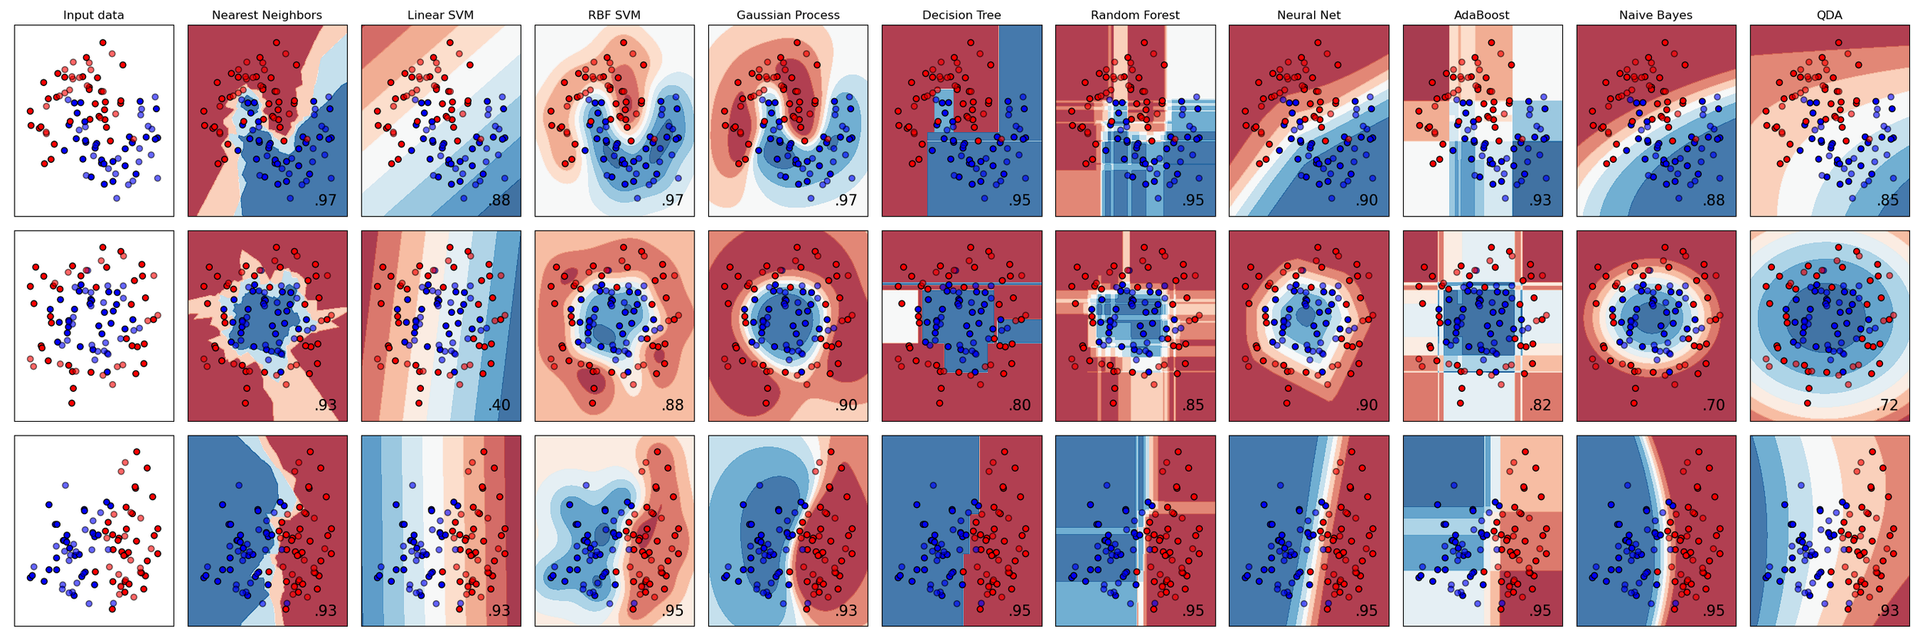
\includegraphics[width=5cm]{figures/img_p001_01.png}}

\begin{document}

% ============================================================ A1-A3 apertura
\titleframe
\addtocounter{framenumber}{1}

\begin{frame}{Contenido}
  \begin{columns}[T]
    \begin{column}{0.9\textwidth}
      \small\tableofcontents
    \end{column}
  \end{columns}
\end{frame}

\begin{frame}{Dónde quedamos}
  \begin{columns}[T]
    \begin{column}{0.5\textwidth}
      \colhead{Ayer (S5)}
      \footnotesize
      \begin{itemize}
        \item 1.740 vendedores de Olist, 8 variables, log + escalado;
        \item PCA: tamaño (PC1) y mala entrega (PC2);
        \item t-SNE y UMAP: vecindarios, no distancias globales.
      \end{itemize}
      \vspace{4pt}
      \colhead{Hoy}
      \begin{itemize}
        \item proponer \textbf{grupos} en ese espacio y decidir si sirven;
        \item lo que no encaja (outliers) y lo que cambia (drift).
      \end{itemize}
    \end{column}
    \begin{column}{0.44\textwidth}
      \begin{keybox}[Taller, Módulo C]
        \small Entrega 17/10. K-Means + otra familia, codo, silueta, Davies--Bouldin, ARI entre semillas y perfiles con acción. Todo eso aparece hoy, con vendedores en lugar de clientes.
      \end{keybox}
    \end{column}
  \end{columns}
\end{frame}

% ============================================================ 1. formular
\section{Formular el clustering}
\sectionframe{Formular el clustering}

\begin{frame}{Un cluster no es un segmento}
  \begin{columns}[T]
    \begin{column}{0.48\textwidth}
      \begin{defbox}[Cluster]
        \small Lo que entrega el algoritmo: una partición de los datos que optimiza un criterio geométrico.
      \end{defbox}
      \small Cualquier algoritmo con $k=4$ devuelve 4 grupos, \textbf{haya o no estructura}.
      \begin{rulebox}
        \small Siempre hay clusters. No siempre hay segmentos.
      \end{rulebox}
    \end{column}
    \begin{column}{0.48\textwidth}
      \begin{defbox}[Segmento]
        \footnotesize Un grupo que el negocio puede usar. Debe ser:
        \begin{itemize}
          \item \textbf{nombrable}: se describe en una frase;
          \item \textbf{estable}: sobrevive a otra semilla o muestra;
          \item \textbf{accionable}: pide una acción distinta;
          \item \textbf{de tamaño útil}: ni el 85\,\% ni 12 casos.
        \end{itemize}
      \end{defbox}
    \end{column}
  \end{columns}
\end{frame}

\begin{frame}{La distancia define los grupos}
  \small El clustering agrupa lo que está \textbf{cerca}. Quien decide qué es ``cerca'' es usted:
  \begin{columns}[T]
    \begin{column}{0.48\textwidth}
      \begin{goldbox}[Qué variables]
        \footnotesize Con solo ventas y órdenes, los grupos serán ``grandes'' y ``pequeños''. Con retraso y calificación aparece la experiencia de entrega.
      \end{goldbox}
      \begin{goldbox}[Qué escala]
        \footnotesize Sin log ni escalado, ventas (hasta 500.000 BRL) decide sola (S5).
      \end{goldbox}
    \end{column}
    \begin{column}{0.48\textwidth}
      \begin{rulebox}[Variable casi constante]
        \footnotesize En Olist la gran mayoría de los clientes compra \textbf{una sola vez}: la frecuencia vale 1 para casi todos y no separa a nadie. Tras escalar, sus pocos valores distintos de 1 quedan como outliers.
      \end{rulebox}
      \begin{keybox}
        \footnotesize Opciones: binarizar (1 frente a $\geq 2$), sacarla del clustering o usarla solo para perfilar.
      \end{keybox}
    \end{column}
  \end{columns}
\end{frame}

\begin{frame}{Cuatro familias}
  \centering\footnotesize
  \begin{tabular}{@{}L{0.17\textwidth} L{0.2\textwidth} L{0.26\textwidth} L{0.27\textwidth}@{}}
    \toprule
    \hrow \textbf{Familia} & \textbf{Ejemplos} & \textbf{Qué supone} & \textbf{Dónde falla} \\
    \midrule
    Centroides & K-Means, Mini-Batch & grupos convexos, de tamaño y varianza parecidos & formas alargadas o curvas; outliers \\
    Jerárquica & aglomerativo (Ward, average, single) & depende del linkage & $n$ grande (memoria $O(n^2)$) \\
    Densidad & DBSCAN, HDBSCAN & grupos = zonas densas separadas por zonas ralas & datos sin zonas ralas; muchas dimensiones \\
    Modelos & GMM & mezcla de gaussianas & solo mención hoy \\
    \bottomrule
  \end{tabular}
  \raggedright
  \begin{keybox}
    \small Cada familia trae su propia idea de ``grupo''. Elegir el algoritmo es elegir esa idea.
  \end{keybox}
\end{frame}

% ============================================================ 2. K-Means
\section{K-Means y Mini-Batch K-Means}
\sectionframe{K-Means}

\begin{frame}{El objetivo}
  \small Dado $k$, buscar centroides $\mu_1,\dots,\mu_k$ y asignaciones $C_1,\dots,C_k$ que minimicen la \textbf{inercia}:
  \[ J = \sum_{c=1}^{k} \sum_{i \in C_c} \lVert x_i - \mu_c \rVert^2 \]
  \begin{columns}[T]
    \begin{column}{0.48\textwidth}
      \begin{defbox}[Algoritmo de Lloyd]
        \small Repetir hasta que nada cambie:
        \begin{enumerate}
          \item \textbf{asignar}: cada punto al centroide más cercano;
          \item \textbf{actualizar}: cada centroide = media de sus puntos.
        \end{enumerate}
      \end{defbox}
    \end{column}
    \begin{column}{0.48\textwidth}
      \begin{goldbox}[Garantías]
        \small Cada paso baja $J$ (o la deja igual), así que converge. Pero encontrar el mínimo global es NP-hard: Lloyd llega a un \textbf{mínimo local} que depende del inicio.
      \end{goldbox}
    \end{column}
  \end{columns}
\end{frame}

\begin{frame}{Lloyd a mano: el mini-mundo}
  \begin{columns}[c]
    \begin{column}{0.34\textwidth}
      \centering
      \begin{tikzpicture}[scale=0.3]
        \miniaxes
        \foreach \n/\x/\y in {A/1/2,C/2/3}{\fill[eafitblue] (\x,\y) circle (5pt); \node[font=\tiny,above left] at (\x,\y) {\n};}
        \foreach \n/\x/\y in {B/2/1}{\fill[mlred] (\x,\y) circle (5pt); \node[font=\tiny,below right] at (\x,\y) {\n};}
        \foreach \n/\x/\y in {D/6/5,E/7/7,F/8/6}{\fill[mlgray] (\x,\y) circle (5pt); \node[font=\tiny,above left] at (\x,\y) {\n};}
        \node[font=\scriptsize,anchor=north] at (4.5,-0.4) {inicio: centroides en A y B};
      \end{tikzpicture}\\[4pt]
      \begin{tikzpicture}[scale=0.3]
        \miniaxes
        \foreach \x/\y in {1/2,2/1,2/3}{\fill[eafitblue] (\x,\y) circle (5pt);}
        \foreach \x/\y in {6/5,7/7,8/6}{\fill[mlred] (\x,\y) circle (5pt);}
        \draw[thick] (1.67,2) node[cross out,draw,inner sep=3pt]{};
        \draw[thick] (7,6) node[cross out,draw,inner sep=3pt]{};
        \node[font=\scriptsize,anchor=north] at (4.5,-0.4) {final: $J = 6{,}67$};
      \end{tikzpicture}
    \end{column}
    \begin{column}{0.64\textwidth}
      \footnotesize
      \begin{tabular}{@{}c L{0.3\textwidth} L{0.42\textwidth}@{}}
        \toprule
        \hrow \textbf{Iter.} & \textbf{Asignar} & \textbf{Actualizar} \\
        \midrule
        1 & \{A, C, E\} / \{B, D, F\} & $\mu_1 = (3{,}33;\ 4{,}00)$, $\mu_2 = (5{,}33;\ 4{,}00)$ \\
        2 & \{A, B, C\} / \{D, E, F\} & $\mu_1 = (1{,}67;\ 2{,}00)$, $\mu_2 = (7{,}00;\ 6{,}00)$ \\
        3 & sin cambios & converge \\
        \bottomrule
      \end{tabular}
      \vspace{6pt}

      \footnotesize Aun empezando con los dos centroides en el mismo grupo, Lloyd se recupera porque los grupos están muy separados. Con datos reales no siempre pasa.
      \begin{keybox}
        \footnotesize Ejercicio: verifique $J$ a mano. {\color{mlgray}(Cada grupo aporta 3,33.)}
      \end{keybox}
    \end{column}
  \end{columns}
\end{frame}

\begin{frame}{Inicialización: k-means++}
  \begin{columns}[c]
    \begin{column}{0.58\textwidth}
      \figh{0.68}{k3_init.png}
    \end{column}
    \begin{column}{0.4\textwidth}
      \footnotesize
      \begin{defbox}[k-means++]
        \footnotesize Primer centroide al azar; cada siguiente con probabilidad $\propto D(x)^2$, la distancia al centroide más cercano ya elegido. Los inicios quedan repartidos.
      \end{defbox}
      \begin{itemize}
        \item con inicio aleatorio, el 8,5\,\% de 200 semillas termina con inercia más de 5\,\% peor;
        \item \texttt{n\_init=10}: corre 10 veces y se queda con la menor inercia.
      \end{itemize}
    \end{column}
  \end{columns}
\end{frame}

\begin{frame}{Supuestos y fallos}
  \centering\figh{0.48}{k4_failures.png}
  \raggedright\footnotesize
  \begin{columns}[T]
    \begin{column}{0.48\textwidth}
      K-Means corta el espacio en celdas de Voronoi: fronteras \textbf{rectas} a mitad de camino entre centroides. Supone grupos convexos, de varianza y tamaño parecidos.
    \end{column}
    \begin{column}{0.48\textwidth}
      \begin{rulebox}
        \footnotesize Con lunas, grupos alargados o tamaños muy distintos, K-Means da una partición limpia\ldots{} y equivocada.
      \end{rulebox}
    \end{column}
  \end{columns}
\end{frame}

\begin{frame}{Elegir $k$: el codo}
  \begin{columns}[c]
    \begin{column}{0.55\textwidth}
      \fig{k5_elbow.png}
    \end{column}
    \begin{column}{0.43\textwidth}
      \footnotesize
      \begin{itemize}
        \item la inercia \textbf{siempre} baja con $k$: con $k=n$ vale 0;
        \item se busca el punto donde agregar un grupo deja de ayudar mucho;
        \item en los vendedores de Olist no hay un codo nítido (lo normal con datos reales).
      \end{itemize}
      \begin{keybox}
        \footnotesize El codo es una pista, no una regla: se combina con silueta, DB, estabilidad y negocio.
      \end{keybox}
    \end{column}
  \end{columns}
\end{frame}

\begin{frame}{Mini-Batch K-Means}
  \begin{columns}[T]
    \begin{column}{0.52\textwidth}
      \begin{defbox}[Idea]
        \small En cada paso usar un \textbf{lote} aleatorio de $b$ puntos (p. ej. 1.024 o 4.096) en lugar de todos los datos.
      \end{defbox}
      \small Para cada $x$ del lote, con centroide asignado $c$:
      \[ n_c \leftarrow n_c + 1, \qquad \eta = \tfrac{1}{n_c}, \qquad \mu_c \leftarrow (1-\eta)\,\mu_c + \eta\, x \]
      \footnotesize El paso $\eta$ se achica a medida que el centroide acumula puntos: es un promedio móvil, como un descenso de gradiente estocástico.
    \end{column}
    \begin{column}{0.44\textwidth}
      \begin{goldbox}[Costo por iteración]
        \small K-Means: $O(n\,k\,p)$\\
        Mini-Batch: $O(b\,k\,p)$, con $b \ll n$
      \end{goldbox}
      \begin{goldbox}[Datos que no caben en memoria]
        \small \texttt{partial\_fit} recibe los datos por bloques o en flujo.
      \end{goldbox}
    \end{column}
  \end{columns}
\end{frame}

\begin{frame}{K-Means frente a Mini-Batch}
  \centering\figh{0.45}{k7_minibatch.png}
  \raggedright\footnotesize
  \begin{columns}[T]
    \begin{column}{0.48\textwidth}
      \begin{itemize}
        \item en una laptop, el K-Means de scikit-learn (Elkan/Lloyd en paralelo) es \textbf{más rápido} aquí hasta $10^6$ filas;
        \item Mini-Batch pierde entre 0 y 3\,\% de inercia.
      \end{itemize}
    \end{column}
    \begin{column}{0.48\textwidth}
      \begin{keybox}[Cuándo usarlo]
        \footnotesize Datos que no caben en memoria, que llegan en flujo, o $n$ de decenas de millones. No ``porque es más rápido'': mídalo.
      \end{keybox}
    \end{column}
  \end{columns}
\end{frame}

% ============================================================ 3. jerárquico
\section{Clustering jerárquico}
\sectionframe{Clustering jerárquico}

\begin{frame}{Aglomerativo}
  \begin{columns}[c]
    \begin{column}{0.38\textwidth}
      \centering
      \begin{tikzpicture}[scale=0.45]
        \miniaxes
        \foreach \n/\x/\y in {A/1/2,B/2/1,C/2/3,D/6/5,E/7/7,F/8/6}{\fill[mlteal] (\x,\y) circle (5pt); \node[font=\tiny,above left] at (\x,\y) {\n};}
        \draw[eafitblue,thick,rounded corners] (0.5,0.4) rectangle (2.5,3.5);
        \draw[eafitblue,thick,rounded corners] (6.5,5.5) rectangle (8.5,7.5);
        \draw[mlred,thick,rounded corners,dashed] (5.4,4.4) rectangle (8.7,7.7);
      \end{tikzpicture}
    \end{column}
    \begin{column}{0.6\textwidth}
      \small
      \begin{enumerate}
        \item cada punto empieza como su propio cluster;
        \item fusionar los dos clusters más cercanos;
        \item repetir hasta que quede uno.
      \end{enumerate}
      \footnotesize
      \begin{tabular}{@{}c l c@{}}
        \toprule
        \hrow \textbf{Paso} & \textbf{Fusión (single linkage)} & \textbf{Distancia} \\
        \midrule
        1--3 & A con B, A con C, E con F & 1,41 \\
        4 & D con \{E, F\} & 2,24 \\
        5 & \{A, B, C\} con \{D, E, F\} & 4,47 \\
        \bottomrule
      \end{tabular}
      \vspace{4pt}

      \small El resultado no es una partición: es un \textbf{árbol} de particiones anidadas.
    \end{column}
  \end{columns}
\end{frame}

\begin{frame}{Linkage: distancia entre grupos}
  \centering\footnotesize
  \begin{tabular}{@{}l L{0.36\textwidth} L{0.34\textwidth}@{}}
    \toprule
    \hrow \textbf{Linkage} & \textbf{Distancia entre $G$ y $H$} & \textbf{Efecto} \\
    \midrule
    Single & $\min_{i\in G,\,j\in H} d(i,j)$ & encadena: un puente de puntos une dos grupos \\
    Complete & $\max_{i\in G,\,j\in H} d(i,j)$ & grupos compactos; sensible a outliers \\
    Average & promedio de $d(i,j)$ entre todos los pares & término medio \\
    Ward & aumento de la inercia al fusionar $G$ y $H$ & grupos esféricos de tamaño parecido: el más cercano a K-Means \\
    \bottomrule
  \end{tabular}
  \raggedright
  \begin{keybox}
    \small Ward es la opción por defecto para segmentar con variables numéricas escaladas. Single solo si espera grupos con formas alargadas y sin ruido.
  \end{keybox}
\end{frame}

\begin{frame}{Leer y cortar el dendrograma}
  \figh{0.56}{h3_dendrogram.png}
  \small
  \begin{itemize}
    \item altura de cada unión = disimilitud a la que se fusionaron esos grupos;
    \item cortar con una línea horizontal da una partición; un \textbf{salto grande} de altura sugiere dónde cortar;
    \item aquí: 300 vendedores, Ward, corte en 4 grupos.
  \end{itemize}
\end{frame}

\begin{frame}{Costo y uso práctico}
  \begin{columns}[T]
    \begin{column}{0.48\textwidth}
      \begin{goldbox}[Costo]
        \small Matriz de distancias: memoria $O(n^2)$.
        \begin{itemize}
          \item 1.740 vendedores: 1,5 millones de pares, sin problema;
          \item 96.000 clientes de Olist: 4.600 millones de pares, \textbf{no cabe}.
        \end{itemize}
      \end{goldbox}
      \small Salidas: muestra aleatoria, \texttt{connectivity} (solo vecinos), o K-Means con muchos grupos y luego jerárquico sobre los centroides.
    \end{column}
    \begin{column}{0.48\textwidth}
      \begin{keybox}[Para qué sirve]
        \small Ver la \textbf{jerarquía} de segmentos: un grupo grande que se divide en dos subgrupos con acciones distintas. Y elegir $k$ mirando las alturas.
      \end{keybox}
      \begin{rulebox}
        \small Las fusiones son definitivas: un error temprano no se corrige después.
      \end{rulebox}
    \end{column}
  \end{columns}
\end{frame}

% ============================================================ 4. densidad
\section{DBSCAN y HDBSCAN}
\sectionframe{Clustering por densidad}

\begin{frame}{DBSCAN}
  \begin{columns}[c]
    \begin{column}{0.38\textwidth}
      \centering
      \begin{tikzpicture}[scale=0.45]
        \miniaxes
        \foreach \x/\y in {1/2,2/1,2/3}{\fill[eafitblue] (\x,\y) circle (5pt); \draw[eafitblue!40] (\x,\y) circle (2.3);}
        \foreach \x/\y in {6/5,7/7,8/6}{\fill[mlred] (\x,\y) circle (5pt);}
        \fill[mlgray] (5,1) circle (5pt) node[below right,font=\tiny]{G};
        \draw[mlgray,dashed] (5,1) circle (2.3);
      \end{tikzpicture}\\
      {\scriptsize \texttt{eps} = 2,3 · \texttt{min\_samples} = 3}
    \end{column}
    \begin{column}{0.6\textwidth}
      \small Dos parámetros: radio \texttt{eps} y \texttt{min\_samples}.
      \begin{itemize}
        \item \textbf{núcleo}: tiene al menos \texttt{min\_samples} puntos (contándose) a distancia $\leq$ \texttt{eps};
        \item \textbf{borde}: no es núcleo, pero está a $\leq$ \texttt{eps} de un núcleo;
        \item \textbf{ruido}: ninguna de las dos (etiqueta $-1$).
      \end{itemize}
      Un cluster = núcleos conectados entre sí más sus bordes.
      \begin{goldbox}[Mini-mundo + G(5, 1)]
        \footnotesize A--F son núcleo (2 vecinos a $\leq 2{,}24$). El vecino más cercano de G está a 3,0: \textbf{ruido}. Dos clusters, sin pedir $k$.
      \end{goldbox}
    \end{column}
  \end{columns}
\end{frame}

\begin{frame}{Elegir \texttt{eps}}
  \begin{columns}[c]
    \begin{column}{0.55\textwidth}
      \fig{d2_kdistance.png}
    \end{column}
    \begin{column}{0.43\textwidth}
      \small
      \begin{enumerate}
        \item para cada punto, distancia a su $k$-ésimo vecino ($k$ = \texttt{min\_samples});
        \item ordenar de menor a mayor;
        \item \texttt{eps} cerca del codo: a la derecha están los puntos que quedarían como ruido.
      \end{enumerate}
      \begin{rulebox}[Limitación]
        \small Un solo \texttt{eps} supone \textbf{una sola densidad}. Si hay grupos densos y grupos ralos, ningún valor sirve para todos.
      \end{rulebox}
    \end{column}
  \end{columns}
\end{frame}

\begin{frame}{HDBSCAN}
  \centering\figh{0.4}{d3_hdbscan.png}
  \raggedright\footnotesize
  \begin{columns}[T]
    \begin{column}{0.56\textwidth}
      \begin{enumerate}
        \item distancia de alcanzabilidad mutua: $\max\{\text{core}_k(a), \text{core}_k(b), d(a,b)\}$;
        \item árbol de expansión mínima $\rightarrow$ jerarquía para \textbf{todos} los \texttt{eps};
        \item se conservan los clusters que persisten en un rango amplio de densidades.
      \end{enumerate}
    \end{column}
    \begin{column}{0.4\textwidth}
      \begin{goldbox}[En la práctica]
        \scriptsize Un parámetro principal: \texttt{min\_cluster\_size}. Entrega \texttt{probabilities\_} (fuerza de pertenencia). En \texttt{sklearn.cluster.HDBSCAN}.
      \end{goldbox}
    \end{column}
  \end{columns}
\end{frame}

\begin{frame}{El ruido es un resultado}
  \begin{columns}[T]
    \begin{column}{0.48\textwidth}
      \begin{keybox}
        \small La etiqueta $-1$ no es un error del algoritmo. Dice: ``estos puntos no pertenecen claramente a ningún grupo''.
      \end{keybox}
      \small Qué pueden ser:
      \begin{itemize}
        \item outliers reales (sección 7);
        \item casos ``no segmentables'' que merecen tratamiento genérico;
        \item señal de que \texttt{min\_cluster\_size} es muy grande.
      \end{itemize}
    \end{column}
    \begin{column}{0.48\textwidth}
      \begin{rulebox}[Reporte siempre]
        \small
        \begin{itemize}
          \item qué porcentaje es ruido;
          \item cómo cambia con los parámetros;
          \item qué se hará con esos casos en producción.
        \end{itemize}
      \end{rulebox}
      \small Un 40\,\% de ruido no es ``4 segmentos'': es 4 segmentos \textbf{más} un grupo enorme sin segmentar.
    \end{column}
  \end{columns}
\end{frame}

\begin{frame}{Cuatro algoritmos, mismos datos}
  \begin{columns}[c]
    \begin{column}{0.52\textwidth}
      \centering\figh{0.86}{d5_grid.png}
    \end{column}
    \begin{column}{0.46\textwidth}
      \footnotesize
      \begin{itemize}
        \item \textbf{blobs}: todos aciertan;
        \item \textbf{lunas}: solo los de densidad;
        \item \textbf{anisotrópico}: nadie perfecto; HDBSCAN marca como ruido la zona ambigua;
        \item \textbf{densidad variable}: K-Means y Ward aciertan; DBSCAN con un solo \texttt{eps} deja ruido en el grupo ralo.
      \end{itemize}
      \begin{keybox}
        \footnotesize No hay ganador universal. Compare al menos dos familias.
      \end{keybox}
      {\footnotesize\color{mlgray} Gris = ruido.}
    \end{column}
  \end{columns}
\end{frame}

% ============================================================ 5. validar
\section{Validar sin etiquetas}
\sectionframe{Validar sin etiquetas}

\begin{frame}{Silueta}
  \[ s(i) = \frac{b(i) - a(i)}{\max\{a(i),\, b(i)\}} \in [-1, 1] \]
  \begin{columns}[T]
    \begin{column}{0.48\textwidth}
      \small
      \begin{itemize}
        \item $a(i)$: distancia media de $i$ a su propio cluster (cohesión);
        \item $b(i)$: distancia media al cluster vecino más cercano (separación);
        \item cerca de 1: bien asignado; cerca de 0: en la frontera; negativo: mal asignado.
      \end{itemize}
    \end{column}
    \begin{column}{0.48\textwidth}
      \begin{goldbox}[Mini-mundo, punto A]
        \small $a(A) = \frac{1{,}41 + 1{,}41}{2} = 1{,}41$\\[2pt]
        $b(A) = \frac{5{,}83 + 7{,}81 + 8{,}06}{3} = 7{,}23$\\[2pt]
        $s(A) = \frac{7{,}23 - 1{,}41}{7{,}23} = \mathbf{0{,}80}$
      \end{goldbox}
      \footnotesize La silueta global es el promedio de $s(i)$.
    \end{column}
  \end{columns}
\end{frame}

\begin{frame}{El gráfico de silueta}
  \begin{columns}[c]
    \begin{column}{0.55\textwidth}
      \fig{v2_silhouette.png}
    \end{column}
    \begin{column}{0.43\textwidth}
      \small
      \begin{itemize}
        \item una barra por punto, agrupadas por cluster;
        \item grosor = tamaño del cluster;
        \item valores negativos = puntos que estarían mejor en otro grupo.
      \end{itemize}
      \begin{keybox}[Vendedores de Olist]
        \small Silueta media 0,20: los grupos existen pero se tocan. Es lo habitual con comportamiento de clientes o vendedores: más un continuo que islas.
      \end{keybox}
    \end{column}
  \end{columns}
\end{frame}

\begin{frame}{Davies--Bouldin y Calinski--Harabasz}
  \centering\footnotesize
  \begin{tabular}{@{}l L{0.36\textwidth} c L{0.24\textwidth}@{}}
    \toprule
    \hrow \textbf{Métrica} & \textbf{Fórmula} & \textbf{Mejor} & \textbf{Ojo} \\
    \midrule
    Silueta & promedio de $\frac{b(i)-a(i)}{\max(a,b)}$ & mayor & costo $O(n^2)$ \\[3pt]
    Davies--Bouldin & $\frac{1}{k}\sum_c \max_{c'\neq c} \frac{s_c + s_{c'}}{d(\mu_c, \mu_{c'})}$ & menor & usa centroides \\[3pt]
    Calinski--Harabasz & $\frac{\operatorname{tr}(B)/(k-1)}{\operatorname{tr}(W)/(n-k)}$ & mayor & crece con grupos esféricos \\
    \bottomrule
  \end{tabular}
  \raggedright
  \vspace{2pt}

  \footnotesize $s_c$: distancia media de los puntos de $c$ a su centroide. $B$, $W$: dispersión entre y dentro de grupos.
  \begin{keybox}
    \small Las tres miden lo mismo con otra fórmula: grupos compactos y separados. Ninguna mide si el grupo sirve.
  \end{keybox}
\end{frame}

\begin{frame}{Las métricas internas prefieren esferas}
  \begin{columns}[c]
    \begin{column}{0.58\textwidth}
      \fig{v4_moons.png}
    \end{column}
    \begin{column}{0.4\textwidth}
      \small
      \begin{itemize}
        \item DBSCAN encuentra las dos lunas;
        \item K-Means las corta mal\ldots{}
        \item \ldots{} y aun así tiene \textbf{mejor silueta} (0,50 frente a 0,39).
      \end{itemize}
      \begin{rulebox}
        \small Silueta, DB y CH asumen grupos compactos. No compare con ellas algoritmos de familias distintas sin mirar los datos.
      \end{rulebox}
      \footnotesize Con ruido: calcule la métrica sin los $-1$ y reporte el \% de ruido aparte.
    \end{column}
  \end{columns}
\end{frame}

\begin{frame}{Estabilidad: ARI}
  \begin{columns}[c]
    \begin{column}{0.52\textwidth}
      \fig{v5_ari_box.png}
    \end{column}
    \begin{column}{0.46\textwidth}
      \small
      \begin{enumerate}
        \item tomar submuestras del 80\,\% (o cambiar la semilla);
        \item reajustar y comparar con la partición completa;
        \item \emph{Adjusted Rand Index}: 1 = mismas particiones, 0 = coincidencia al azar.
      \end{enumerate}
      \begin{defbox}[Stability index]
        \footnotesize ARI medio entre réplicas (Ben-Hur et al., 2002; Lange et al., 2004). Un $k$ que no se repite no describe los datos.
      \end{defbox}
      \footnotesize \texttt{sklearn.metrics.adjusted\_rand\_score}
    \end{column}
  \end{columns}
\end{frame}

\begin{frame}{Decidir $k$ con evidencia}
  \centering\scriptsize\renewcommand{\arraystretch}{1.0}
  \begin{tabular}{@{}c r c c r c c@{}}
    \toprule
    \hrow $k$ & \textbf{Inercia} & \textbf{Silueta} $\uparrow$ & \textbf{DB} $\downarrow$ & \textbf{CH} $\uparrow$ & \textbf{ARI medio} $\uparrow$ & \textbf{Grupo más chico} \\
    \midrule
    2 & 11.244 & 0,185 & 1,88 & \textbf{414} & \textbf{0,97} & 47\,\% \\
    \rowcolor{eafitsky!40} 3 & 9.533 & \textbf{0,202} & 1,59 & 400 & 0,87 & 18\,\% \\
    4 & 8.319 & 0,177 & \textbf{1,53} & 390 & 0,88 & 12\,\% \\
    5 & 7.639 & 0,174 & 1,56 & 357 & 0,85 & 11\,\% \\
    6 & 7.138 & 0,157 & 1,56 & 330 & 0,89 & 10\,\% \\
    7 & 6.720 & 0,164 & 1,58 & 309 & 0,88 & 8\,\% \\
    8 & 6.396 & 0,169 & 1,55 & 291 & 0,80 & 5\,\% \\
    \bottomrule
  \end{tabular}\par
  \vspace{6pt}
  \raggedright
  \begin{columns}[T]
    \begin{column}{0.48\textwidth}
      \footnotesize Las métricas \textbf{no coinciden}. $k=2$ es el más estable pero dice poco; $k=3$ y $k=4$ quedan casi empatados.
    \end{column}
    \begin{column}{0.48\textwidth}
      \begin{keybox}[Elección: $k=3$]
        \footnotesize Mejor silueta y CH (salvo $k=2$), ARI 0,87, ningún grupo $<$ 15\,\% y tres acciones distintas. Con $k=4$ habría que mostrar que el cuarto grupo pide otra acción.
      \end{keybox}
    \end{column}
  \end{columns}
\end{frame}

% ============================================================ 6. segmentación
\section{Segmentación accionable}
\sectionframe{De cluster a segmento}

\begin{frame}{El pipeline completo}
  \centering
  \begin{tikzpicture}[node distance=0.22cm,
      st/.style={fill=mlcream,minimum height=1cm,align=center,font=\scriptsize,text width=1.45cm},
      arr/.style={-{Stealth[length=1.6mm]},thick,eafitblue}]
    \node[st] (a) {SQL:\\features};
    \node[st,right=of a] (b) {log +\\escalado};
    \node[st,right=of b,fill=eafitsky] (c) {(PCA)};
    \node[st,right=of c,fill=eafitsky] (d) {clustering};
    \node[st,right=of d] (e) {validar:\\métricas + ARI};
    \node[st,right=of e] (f) {perfilar en variables originales};
    \node[st,right=of f,fill=mlgold!30] (g) {nombrar y actuar};
    \foreach \u/\v in {a/b,b/c,c/d,d/e,e/f,f/g}{\draw[arr] (\u) -- (\v);}
  \end{tikzpicture}
  \vspace{8pt}
  \raggedright
  \begin{columns}[T]
    \begin{column}{0.48\textwidth}
      \begin{goldbox}[Con qué datos]
        \small Features con información hasta la fecha de corte (aquí 2018-06-01). Para asignar vendedores nuevos: \texttt{predict} del mismo pipeline, sin reajustar.
      \end{goldbox}
    \end{column}
    \begin{column}{0.48\textwidth}
      \begin{rulebox}[Las proyecciones 2D]
        \small t-SNE y UMAP en 2D sirven para \textbf{mirar} los grupos. No se agrupa sobre ellas (S5).
      \end{rulebox}
    \end{column}
  \end{columns}
\end{frame}

\begin{frame}{Perfilamiento}
  \centering\figh{0.62}{s2_profiles.png}\par
  \raggedright\footnotesize Mediana de cada variable por grupo. Color: cuántas veces la mediana del grupo supera (naranja) o queda por debajo (azul) de la mediana global. Se perfila en las \textbf{variables originales}, no en las escaladas.
\end{frame}

\begin{frame}{Nombrar y actuar}
  \centering\footnotesize
  \begin{tabular}{@{}L{0.22\textwidth} L{0.36\textwidth} L{0.32\textwidth}@{}}
    \toprule
    \hrow \textbf{Segmento} & \textbf{Evidencia (mediana)} & \textbf{Acción} \\
    \midrule
    \textbf{C0 · Grandes y diversificados} (735) & 43 órdenes, 5,9 k BRL, 3 categorías, 7\,\% de retraso & cuenta clave: soporte dedicado, prioridad en campañas \\
    \textbf{C1 · Con problemas de entrega} (318) & 25\,\% de retraso, 3,6 días hasta la transportadora, calificación 3,65 & plan logístico, alertas de despacho, seguimiento de reseñas \\
    \textbf{C2 · Pequeños de ticket bajo} (687) & ticket 74 BRL, flete = 27\,\% del precio, 0\,\% de retraso, calificación 4,39 & subsidio o consolidación de flete; incentivos para crecer \\
    \bottomrule
  \end{tabular}
  \raggedright
  \begin{keybox}
    \small Cada nombre debe poder leerse en la tabla de perfiles. Si dos segmentos terminan con la misma acción, para el negocio son uno solo.
  \end{keybox}
\end{frame}

\begin{frame}{Práctica: ¿aprobaría esta segmentación?}
  \begin{taskbox}[Situación]
    \small Un equipo presenta 5 segmentos de clientes con silueta 0,55. En el anexo: ARI medio entre semillas 0,40, y un segmento tiene el 85\,\% de los clientes. Las otras cuatro campañas apuntan al 15\,\% restante.
  \end{taskbox}
  \small Discuta en parejas (3 minutos):
  \begin{itemize}
    \item ¿la silueta alta compensa el ARI bajo?
    \item ¿qué dice un grupo con el 85\,\%?
    \item ¿qué pediría antes de aprobar?
  \end{itemize}
  \begin{keybox}[Respuesta esperada]
    \small No se aprueba. ARI 0,40 = otra semilla da otros segmentos. El 85\,\% sugiere que la silueta alta viene de separar unos pocos casos raros (¿outliers?). Pedir: estabilidad, perfiles y otra familia de algoritmos.
  \end{keybox}
\end{frame}

\begin{frame}{Anti-patrones}
  \begin{columns}[T]
    \begin{column}{0.54\textwidth}
      \small
      \begin{enumerate}
        \item elegir $k$ solo por silueta (o solo por el codo);
        \item agrupar sobre t-SNE o UMAP en 2D;
        \item no escalar, o escalar sin transformar las sesgadas;
        \item no probar otras semillas ni submuestras;
        \item segmentos sin una acción distinta;
        \item un grupo gigante y varios diminutos;
        \item perfilar en variables escaladas (``z = 1,3'' no le dice nada a nadie).
      \end{enumerate}
    \end{column}
    \begin{column}{0.42\textwidth}
      \begin{rulebox}
        \small Cualquiera de estos invalida una segmentación aunque las métricas se vean bien.
      \end{rulebox}
      \begin{keybox}[Taller]
        \small La rúbrica del Módulo C evalúa estabilidad y perfilamiento accionable, no solo el número de grupos.
      \end{keybox}
    \end{column}
  \end{columns}
\end{frame}

% ============================================================ 7. outliers
\section{Outliers: Isolation Forest y LOF}
\sectionframe{Lo que no encaja: outliers}

\begin{frame}{Isolation Forest}
  \begin{columns}[c]
    \begin{column}{0.4\textwidth}
      \centering
      \begin{tikzpicture}[scale=0.45]
        \miniaxes
        \foreach \x/\y in {1/2,2/1,2/3,6/5,7/7,8/6}{\fill[mlteal] (\x,\y) circle (5pt);}
        \fill[mlred] (5,1) circle (5pt) node[below right,font=\tiny]{G};
        \draw[mlgold,thick] (4.2,0) -- (4.2,8) node[above,font=\tiny]{1};
        \draw[mlgold,thick] (4.2,3.6) -- (9,3.6) node[right,font=\tiny]{2};
      \end{tikzpicture}\\
      {\scriptsize G queda aislado con 2 cortes}
    \end{column}
    \begin{column}{0.58\textwidth}
      \footnotesize
      \begin{itemize}
        \item árboles con cortes \textbf{aleatorios} (variable al azar, umbral al azar);
        \item un punto raro queda solo en una hoja con \textbf{pocos} cortes; uno normal necesita muchos;
        \item score con la profundidad media $E[h(x)]$ en el bosque:
      \end{itemize}
      \[ s(x) = 2^{-E[h(x)]/c(n)} \]
      {\footnotesize $c(n)$: profundidad media esperada. $s \to 1$: anómalo; $s \approx 0{,}5$: normal.}
      \begin{goldbox}[Parámetro clave]
        \scriptsize \texttt{contamination}: qué fracción se marca como anómala. Es una decisión de negocio.
      \end{goldbox}
    \end{column}
  \end{columns}
\end{frame}

\begin{frame}{Local Outlier Factor}
  \begin{columns}[c]
    \begin{column}{0.56\textwidth}
      \fig{o2_if_vs_lof.png}
    \end{column}
    \begin{column}{0.42\textwidth}
      \small LOF compara la densidad local de un punto con la de sus $k$ vecinos:
      \begin{itemize}
        \item LOF $\approx 1$: tan denso como su vecindario;
        \item LOF $\gg 1$: mucho más aislado que sus vecinos.
      \end{itemize}
      \footnotesize El punto (1,2; 1,2) está cerca del grupo denso: LOF = 3,5 (anómalo); para Isolation Forest es el nº 30 de 403.
      \vspace{2pt}
      \begin{keybox}
        \footnotesize IF: raro respecto a \textbf{todos}. LOF: raro respecto a \textbf{sus vecinos}.
      \end{keybox}
    \end{column}
  \end{columns}
\end{frame}

\begin{frame}{Práctica: el 1\,\% más raro}
  \begin{columns}[T]
    \begin{column}{0.5\textwidth}
      \small Con \texttt{contamination=0.01} sobre los 1.740 vendedores:
      \begin{itemize}
        \item Isolation Forest marca 18, LOF marca 18;
        \item solo \textbf{7} aparecen en ambos;
        \item mediana de los marcados por IF: 53\,\% de retraso, 9,1 días hasta la transportadora, flete = 50\,\% del precio, calificación 2,67.
      \end{itemize}
    \end{column}
    \begin{column}{0.46\textwidth}
      \begin{taskbox}[¿Qué hace con ellos?]
        \small Para cada uno decida: ¿error de datos?, ¿vendedor con problemas operativos?, ¿fraude?, ¿vendedor excepcional?
      \end{taskbox}
      \begin{rulebox}
        \small Un outlier se investiga antes de borrarlo. Muchas veces es el caso más importante del dataset.
      \end{rulebox}
    \end{column}
  \end{columns}
\end{frame}

% ============================================================ 8. confiabilidad
\section{Confiabilidad: drift y calibración}
\sectionframe{Cuando el mundo cambia}

\begin{frame}{Tipos de drift}
  \centering\figh{0.28}{r1_late_monthly.png}\par
  \scriptsize\renewcommand{\arraystretch}{1.08}
  \begin{tabular}{@{}l L{0.22\textwidth} L{0.44\textwidth}@{}}
    \toprule
    \hrow \textbf{Tipo} & \textbf{Qué cambia} & \textbf{En Olist} \\
    \midrule
    Covariate & $P(X)$ & más órdenes de otras regiones, otro mix de categorías \\
    Prior & $P(y)$ & la tasa de retraso pasa de 3\,\% a 21\,\% (mar.\ 2018) \\
    Concepto & $P(y \mid X)$ & la misma distancia y peso ya no implican el mismo riesgo \\
    Predicción & $P(\hat y)$ & el modelo del Módulo A dispara el triple de alertas \\
    Segmentos & tamaños, centroides & vendedores que migran de C2 a C1 \\
    \bottomrule
  \end{tabular}
\end{frame}

\begin{frame}{Detectarlo: PSI y KS}
  \centering\figh{0.38}{r2_drift.png}\par
  \raggedright\footnotesize
  \begin{columns}[T]
    \begin{column}{0.52\textwidth}
      \[ \text{PSI} = \sum_{b} (a_b - e_b)\,\ln\frac{a_b}{e_b} \]
      {\scriptsize $e_b$, $a_b$: proporción en el bin $b$ en la referencia y en el periodo actual. Regla usual: $<0{,}1$ estable; $0{,}1$--$0{,}25$ vigilar; $>0{,}25$ cambio fuerte.}
    \end{column}
    \begin{column}{0.44\textwidth}
      \scriptsize
      \begin{itemize}
        \item días de entrega: mediana 10,2 $\rightarrow$ 14,0; PSI = 0,34;
        \item plazo prometido: 22,7 $\rightarrow$ 16,4 días; PSI = 0,96;
        \item KS: máxima distancia entre las dos distribuciones acumuladas (\texttt{scipy.stats.ks\_2samp}).
      \end{itemize}
    \end{column}
  \end{columns}
\end{frame}

\begin{frame}{Repaso: calibración y plan de monitoreo}
  \begin{columns}[T]
    \begin{column}{0.36\textwidth}
      \begin{goldbox}[De la S1]
        \footnotesize Un modelo calibrado dice 20\,\% y acierta 1 de cada 5. Se revisa con la curva de confiabilidad y el Brier score; se corrige con Platt o regresión isotónica. Con drift, la calibración se degrada aunque el AUC se mantenga.
      \end{goldbox}
    \end{column}
    \begin{column}{0.6\textwidth}
      \centering\footnotesize
      \begin{tabular}{@{}L{0.26\textwidth} L{0.24\textwidth} L{0.36\textwidth}@{}}
        \toprule
        \hrow \textbf{Qué monitorear} & \textbf{Cómo} & \textbf{Si se dispara} \\
        \midrule
        Features & PSI, KS por variable & revisar el pipeline de datos \\
        Predicciones & PSI de $\hat y$, nº de alertas & revisar el umbral \\
        Calibración & curva y Brier con etiquetas nuevas & recalibrar (isotónica) \\
        Desempeño & PR-AUC, Recall@k & reentrenar \\
        Segmentos & tamaños, migración & reajustar o renombrar \\
        \bottomrule
      \end{tabular}
    \end{column}
  \end{columns}
\end{frame}

% ============================================================ 9. cierre
\section{Cierre del curso}

\begin{frame}{El curso en una página}
  \centering
  \begin{tikzpicture}[node distance=0.18cm,
      st/.style={fill=mlcream,minimum height=1.9cm,align=center,font=\scriptsize,text width=1.85cm},
      arr/.style={-{Stealth[length=1.6mm]},thick,eafitblue}]
    \node[st] (s1) {\textbf{S1}\\evaluar bien\\[2pt]{\color{mlgray}baseline, PR-AUC, umbral}};
    \node[st,right=of s1] (s2) {\textbf{S2}\\boosting y HPO\\[2pt]{\color{mlgray}CV dentro de Optuna}};
    \node[st,right=of s2] (s3) {\textbf{S3}\\el tiempo\\[2pt]{\color{mlgray}walk-forward, sin futuro}};
    \node[st,right=of s3] (s4) {\textbf{S4}\\ranking y SHAP\\[2pt]{\color{mlgray}NDCG, explicar}};
    \node[st,right=of s4] (s5) {\textbf{S5}\\representar\\[2pt]{\color{mlgray}escalado, embeddings}};
    \node[st,right=of s5,fill=eafitsky] (s6) {\textbf{S6}\\estructura y confiabilidad\\[2pt]{\color{mlgray}estable, accionable, vigilado}};
    \foreach \u/\v in {s1/s2,s2/s3,s3/s4,s4/s5,s5/s6}{\draw[arr] (\u) -- (\v);}
  \end{tikzpicture}
  \vspace{8pt}
  \raggedright
  \begin{keybox}[La regla que atraviesa el curso]
    \small Un resultado de ML vale lo que vale la evidencia que lo respalda: validación honesta, baseline, estabilidad y una decisión que cambie gracias a él.
  \end{keybox}
\end{frame}

\begin{frame}{Taller, examen y referencias}
  \begin{columns}[T]
    \begin{column}{0.48\textwidth}
      \begin{taskbox}[Checklist Módulo C]
        \scriptsize
        \begin{itemize}
          \item features por cliente en SQL, hasta 2018-06-01;
          \item frecuencia casi constante: decida qué hacer;
          \item K-Means + otra familia; codo, silueta, DB y negocio;
          \item PCA + UMAP o t-SNE coloreados por segmento;
          \item ARI entre semillas o submuestras;
          \item perfiles, nombres y una acción por segmento.
        \end{itemize}
      \end{taskbox}
      \begin{keybox}[Examen final]
        \scriptsize 20 preguntas de opción múltiple (Interactiva): criterio, no memoria.
      \end{keybox}
    \end{column}
    \begin{column}{0.48\textwidth}
      \scriptsize
      \begin{itemize}
        \item Ester, M. et al. (1996). A density-based algorithm for discovering clusters (DBSCAN). \emph{KDD}.
        \item Campello, R., Moulavi, D. y Sander, J. (2013). Density-based clustering based on hierarchical density estimates. \emph{PAKDD}.
        \item Liu, F. T., Ting, K. M. y Zhou, Z.-H. (2008). Isolation Forest. \emph{ICDM}.
        \item Breunig, M. et al. (2000). LOF: identifying density-based local outliers. \emph{SIGMOD}.
        \item Hubert, L. y Arabie, P. (1985). Comparing partitions. \emph{J. Classification}.
        \item Ben-Hur, A., Elisseeff, A. y Guyon, I. (2002). A stability based method for discovering structure in clustered data. \emph{PSB}.
        \item scikit-learn. Clustering; Novelty and outlier detection.
      \end{itemize}
    \end{column}
  \end{columns}
\end{frame}

\begin{frame}[plain]
  \begin{tikzpicture}[remember picture,overlay]
    \node[anchor=north west,inner sep=0pt] at ([xshift=309pt,yshift=-45pt]current page.north west)
      {
\includegraphics[width=117pt]{figures/img_p139_45.png}};
    \node[anchor=north west,inner sep=0pt] at ([xshift=177pt,yshift=-191pt]current page.north west)
      {
\includegraphics[width=96pt]{figures/img_p139_46.png}};
    \node[anchor=center,align=center] at ([xshift=158pt,yshift=-90pt]current page.north west)
      {{\color{mltitle}\LARGE\bfseries Gracias por su atención}\\[6pt]
       {\color{mltitle}\normalsize ¿Preguntas, comentarios o discusión?}};
    \node[anchor=north,align=center,font=\footnotesize] at ([xshift=227pt,yshift=-143pt]current page.north west)
      {\textbf{Aprendizaje Automático}\\
       SI7009 · Universidad EAFIT};
  \end{tikzpicture}
\end{frame}

\end{document}
